%%%%%%%%%%%%%%%%%%%%%%%%%%%%%%%%%%%%%%%%%%%%%%%%%%%%%%%%%%%%%%%%
%%%%%%%%%%%%%%%%%%%%%%%%%%%%%%%%%%%%%%%%%%%%%%%%%%%%%%%%%%%%%%%%

%% This is a LaTeX template for writing Project/Seminar Reports of the B.Tech/M Tech Programmes of APJAKTU. 

%% The template was developed by
%%     Dr. Sheena N.
%%     Assistant Professor
%%     Department of Computer Science and Engineering
%%     College of Engineering and Management Punnapra
%%     Alappuzha
%% Customized for CSE department, College of Engineering and Management Punnapra, Alappuzha 

%%%%%%%%%%%%%%%%%%%%%%%%%%%%%%%%%%%%%%%%%%%%%%%%%%%%%%%%%%%%%%%%
%%%%%%%%%%%%%%%%%%%%%%%%%%%%%%%%%%%%%%%%%%%%%%%%%%%%%%%%%%%%%%%%




\documentclass[12pt,a4paper]{report}
\usepackage{graphicx}
\usepackage{amsmath}
\usepackage{fancyhdr}
\usepackage{cite}
\usepackage{framed}
\usepackage{a4wide}
\usepackage{float}
\usepackage{epsfig}
\usepackage{longtable}
\usepackage{enumerate}
\usepackage{afterpage}
\usepackage{multirow}
\usepackage{ragged2e}
\usepackage{gensymb}
\usepackage{amsfonts} 
\usepackage[left=3.5cm,top=3cm,right=3cm,bottom=3cm]{geometry}
\usepackage{setspace}           
\usepackage{float}
\usepackage{txfonts}
\usepackage{lipsum}
\usepackage[T1]{fontenc}
\usepackage{titlesec}
\usepackage{calc} 
\usepackage[titles]{tocloft}
\usepackage{apptools, etoolbox}
\usepackage[title]{appendix}
\usepackage[utf8]{inputenc}
\usepackage{fancyhdr}


\usepackage{tocloft,calc,\renewcommand{\cftchappresnum }{\chaptername\space and \setlength{\cftchapnumwidth}{\widthof{\textbf{Appendix~999~}}}}

\usepackage{lscape} % for landscape tables
\renewcommand{\baselinestretch}{1.7} 

\usepackage{blindtext}
\usepackage{xpatch}
\usepackage{url}
\usepackage{leqno}
\usepackage{subcaption}

\linespread{1.5}
\usepackage[intoc, english]{nomencl}
\hyphenpenalty=5000
\tolerance=1000
\usepackage[nottoc]{tocbibind}

\titleformat{\chapter}[display]{\bfseries\filcenter}{\huge\chaptername~\thechapter}{6ex}{\Huge\thispagestyle{empty}}

\def\listofpapers{
           \normalbaselines
           \chapter*{\centerline{LIST OF PUBLICATIONS}}
           \markboth{LIST OF PUBLICATIONS}{LIST OF PUBLICATIONS}
           \addcontentsline{toc}{chapter}{LIST OF PUBLICATIONS}
   }
% ******* References config *********
\bibliographystyle{IEEEtran}   % On some TeX systems this works
%\bibliographystyle{ieeetr}      % While on others this works
							% Uncomment and test if your references don't cite
							% correctly

%******************************************************************
\renewcommand{\bibname}{REFERENCES}
\renewcommand\contentsname{\centering TABLE OF CONTENTS}
\renewcommand\listfigurename{ LIST OF FIGURES}
\renewcommand\listtablename{ LIST OF TABLES}
\renewcommand{\chaptername}{CHAPTER}
\renewcommand{\appendixname}{APPENDIX}
\newcommand{\Usefont}[1]{\fontfamily{#1}\selectfont}

%********************* Header and Footer*************************
\pagestyle{fancy}
\fancyhf{}

\fancyhead[L]{\slshape Chapter \thechapter} 

\fancyhead[R]{\nouppercase{ \slshape \footnotesize \leftmark}} 
\renewcommand{\chaptermark}[1]{\markboth{#1}{#1}}

\fancyfoot[R]{\slshape \thepage}
\fancyfoot[L]{\slshape \footnotesize  \title}
\renewcommand\footrule{\hrule width1\textwidth height1pt}
\renewcommand\arraystretch{1.5}


%*********************Figures*****************************
% Save all figures in the folder figures and include them in your 
% report using the command \includegraphics{figure-name}

\graphicspath{{figures/}}

% figure files can be in jpeg,jpg, png or pdf formats
%*******************************************************************


\begin{document}
	
	
%****The entries in this section are to be filled in by the student with appropriate values *************

% These values are used thoroughout the report 
% please fill in the appropriate values in the brackets {}

\gdef \title{How to prepare a Technical report using \LaTeX } % Project title
%\gdef \author{Student Name}	 %student name
\gdef \dept{Computer Science and Engineering} %Department
\gdef \degree{Bachelor of Technology} %degree
\gdef \branch{Computer Science and Engineering} %branch
\gdef \college{College of Engineering and Management Punnapra} % Name of the College
\gdef \collegeplace{Alappuzha} % Location of the College
\gdef \studentA{Group member 1} %Project batch member 1
\gdef \studentAroll{Group member1 KTU IDo} % Project batch member 1 ktu id
\gdef \studentB{Group member 2} %Project batch member 2
\gdef \studentBroll{Group member2 KTU ID} % Project batch member 2 ktu id

\gdef \studentC{Group member 3} %Project batch member 3
\gdef \studentCroll{Group member3 KTU ID} % Project batch member 3 ktu id

\gdef \studentD{Group member 4} %Project batch member 4
\gdef \studentDroll{Group member4 KTU ID} % Project batch member 4 ktu id
\gdef \author{Student name} %Name of student for seminar
\gdef \rollno{Student KTU ID} % Roll number of studentfor semnar
\gdef \guide{Dr. Sheena N.} %Project guide
\gdef \guidedes{Assistant Professor}%project guide designation

\gdef \guideco{Prof. Project coguide} %Project coguide
\gdef \guidecodes{Assistant Professor}%project coguide designation

\gdef \guideext{Prof. Project ext guide} %Project external organisation guide
\gdef \guideextdes{Engineer/Scientist}%project external guide designation
\gdef \guideextorg{External guide organization} % Project external guide organization

\gdef \projcordinatorA{Dr. Sheena N.}% Project coordinator 1 
\gdef \projcordinatorAdes{Assistant Professor}% Project coordinator 1 designation

\gdef \semcordinatorA{Prof. Seminar coordinator} % Project coordinator 2 \gdef \projcordinatorBdes{Assistant Professor}% Seminar coordinator 2 designation

\gdef \hod{Suresh Kumar N.} %Head of Department
\gdef \hoddes{Associate Professor \& Head} %HOD designation

\gdef \acadyear{2024 - 25} % Academic year
\gdef \month{Nov 2024} %Month of Report submission
\gdef \date{01-11-2024} %Date of signing the declaration

%*******************************************************************
% The font pages. The source tex files are there in the folder
%======================coverpage.tex================================


\newenvironment{coverpage}
\thispagestyle{empty}
\begin{titlepage}
	\begin{center}
		{\Usefont{phv} \Large \bf \title \par}
		\vspace*{40pt}
		%\large \em \Usefont{pzc}{ 
			\large A PROJECT REPORT \par
			submitted by\\
    
            \vspace{0.5cm}
        \bf {\studentA} (\studentAroll)\\
		\bf {\studentB} (\studentBroll)\\
		\bf {\studentC} (\studentCroll)\\
		\bf {\studentD} (\studentDroll)\\
   
        \vspace{0.5cm}   

       \textnormal{  to \\
  the APJ Abdul Kalam Technological University\\
			in partial fulfillment of requirements for the award of degree\\of}\\ [.15\baselineskip] \par
		\Usefont{ppl} {  \degree}\\
		in\\
		{\Usefont{ppl} {\textit \branch}}\\
  
		
		
		\vspace*{20pt}
		\centering
		\begin{figure}[h!]
		\centerline{
\includegraphics[scale=0.13]{logo-CEMP.jpg}}
		\end{figure}
		
		\vspace{\stretch{0.4}}
		\footnotesize{\bf DEPARTMENT OF COMPUTER SCIENCE AND ENGINEERING} \par
		\bf{COLLEGE OF ENGINEERING AND MANAGEMENT PUNNAPRA} \par
		\bf{ALAPPUZHA} \par
		\bf{\month}
	\end{center}		
\end{titlepage}	
 %Unless essential Do not edit this tex file

%**************************Declaration******************************
%Unless essential Do not edit this tex file

\include{declaration} 

%%********************Certificate*******************
%Unless essential Do not edit this tex file
%  Certificate of project
%===================certificate1.tex================================


\newenvironment{certificate1}

	\newpage
	\begin{center}	
		\textbf{DEPARTMENT OF COMPUTER AND SCIENCE ENGINEERING\\}	
		\textbf{COLLEGE OF ENGINEERING AND MANAGEMENT PUNNAPRA}	
		\textbf{ALAPPUZHA}
	\end{center}
	\begin{figure}[h!]
		\centerline{
\includegraphics[scale=0.1]{logo-CEMP.jpg}}
		\end{figure}
	\begin{center}
		\textbf{CERTIFICATE}
	\end{center}
	
	This is to certify that the report entitled \textbf{\title} submitted by \textbf{\studentA}\hspace*{2pt}(\studentAroll),\hspace*{2pt}\textbf{\studentB}\hspace*{2pt}(\studentBroll),\hspace*{2pt}\textbf{\studentC}\hspace*{2pt}(\studentCroll) \& \textbf{\studentD}\hspace*{2pt}(\studentDroll) to the APJ Abdul Kalam Technological University in partial fulfillment of the requirements for the award of the Degree of Bachelor of Technology in \branch \hspace*{2pt} is a bonafide record of the project work carried out by them under my guidance and supervision. This report in any form has not been submitted to any other University or Institute for any purpose.
	
	
	\begin{singlespace}
		\vspace*{2cm}
		\begin{table}[h!]
			\centering
			\begin{tabular}{p{4.5cm} p{4.5cm} p{5cm}} 
				\textbf{\guide} & \textbf{\projcordinatorA} &\textbf{\hod}\\
				(Project Guide) &  (Project Coordinator) & (Head of Dept.)\\
				\guidedes &  \projcordinatorAdes & \hoddes\\ 
				Dept. of CSE & Dept. of CSE & Dept. of CSE\\ 
				
			\end{tabular}
			
		\end{table}
		
		
	\end{singlespace}
	
	\thispagestyle{empty}



 

%  Certificate of Seminar
%%==================================certificate2.tex================================
% Certificate for Seminar
\newenvironment{certificate2}

\newpage
\begin{center}	
		\textbf{DEPARTMENT OF COMPUTER AND SCIENCE ENGINEERING\\}	
		\textbf{COLLEGE OF ENGINEERING AND MANAGEMENT PUNNAPRA}	
		\textbf{ALAPPUZHA}
\end{center}

\begin{center}
	
\includegraphics[scale=0.1]{logo-CEMP.jpg}	
\end{center}
\begin{center}
	\textbf{CERTIFICATE}
\end{center}

This is to certify that the report entitled \textbf{\title} submitted by \textbf{\author} (\rollno), to the APJ Abdul Kalam Technological University in partial fulfillment of the B.Tech.\ degree in \branch \hspace*{2pt} is a bonafide record of the seminar work carried out by him/her under our guidance and supervision. This report in any form has not been submitted to any other University or Institute for any purpose.

\begin{singlespace}
		\vspace*{2cm}
		\begin{table}[h!]
			\centering
			\begin{tabular}{p{4.5cm} p{4.5cm} p{5cm}} 
				\textbf{\guide} & \textbf{\projcordinatorA} &\textbf{\hod}\\
				(Seminar Guide) &  (Seminar Coordinator) & (Head of Dept.)\\
				\guidedes &  \projcordinatorAdes & \hoddes\\ 
				Dept. of CSE & Dept. of CSE & Dept. of CSE\\ 
				
			\end{tabular}
			
		\end{table}
		
		
	\end{singlespace}



\thispagestyle{empty}



 %Please uncomment this and comment the previous line

%%***************************************************

\pagenumbering{roman} 

%%**********Acknowlegment*****************************************
%Add necessary acknowledgment in the tex file inaddition to the default sentences
% Default Acknowledgement page, Acknowledgement of project
% Please type in the acknowledgement in this tex file  acknowledgement.tex
%===========================acknowledgement.tex======================
\chapter*{\centering ACKNOWLEDGEMENT}%
\addcontentsline{toc}{chapter}{ACKNOWLEDGEMENT}%


\par We express our sincere thanks to \hod, Head of Department,  department of \dept, for providing  us with all the necessary facilities and support.
We would like to express my sincere gratitude to the project coordinator \projcordinatorA,  \projcordinatorAdes,  department of \dept, for the support and co-operation.
We would like to place on record my sincere gratitude to our project guide \guide, \hspace*{2pt}\guidedes, \hspace*{2pt}department of \dept,\hspace*{2pt} %and our external guide \guideext,\hspace*{2pt}\guideextdes, \hspace*{2pt} \guideextorg   
for the guidance and mentorship throughout this work.



\vspace*{30pt}
\begin{flushright}
	\textbf{\studentA}\\
	\textbf{\studentB}\\
	\textbf{\studentC}\\
	\textbf{\studentD}\\
\end{flushright}
\thispagestyle{plain}




%Acknowledgement of seminar

% Please type in the acknowledgement in this tex file  acknowledgement1.tex
%%==================================acknowledgement.tex=============================
\chapter*{Acknowledgement}%
\addcontentsline{toc}{chapter}{Acknowledgement}%




 I express my sincere thanks to \textbf{ \hod}, Head of Department, \dept, for providing  me with all the necessary facilities and support.
I would like to express my sincere gratitude to \textbf{\semcordinatorA},  department of \hspace*{2pt} \dept, \hspace*{2pt} for their support and co-operation
I would like to place on record my sincere gratitude to my seminar guide\hspace*{3pt} \textbf{\guide}, \guidedes, department of \dept, for the guidance and mentorship throughout the course.



\vspace*{30pt}
\begin{flushright}
	\textbf{\author}
\end{flushright}
\thispagestyle{plain}
  

%Please uncomment this and comment the previous line

%%********************************Abstract***********************
 % Please type in the abstract in this tex file abstract.tex
%=======================abstract.tex================================
\chapter*{\centering \uppercase{Abstract}}%
\addcontentsline{toc}{chapter}{\uppercase{Abstract}}

Write the abstract here.Do not exceed 2 pages. No figures, tables, sketches shall be here


\thispagestyle{plain}
%===================================================================




\thispagestyle{empty}
\newpage
    
%%**********************Table of Contents***********************


\tableofcontents

%%*********************List of Tables***********************
\addtocontents{lot}
{\textbf{Table}\hfill\textbf{Title}\hfill\textbf{Page}\par}
\listoftables

%%**********************List of Figures***********************
\addtocontents{lof}
{\textbf{Figure}\hfill\textbf{Title}\hfill\textbf{Page}\par}
\listoffigures


%%**********************Abbreviations***********************
 % Please type in the Abbreviationsin this tex file Abbreviations.tex
%==================================abbreviations.tex================================
% List of Symbols
\chapter*{ABBREVIATIONS}
\addcontentsline{toc}{chapter}{\uppercase{ABBREVIATIONS}}

%Abbrevitaions must be in alphabetical order

\begin{tabular}{p{0.2\linewidth}p{0.8\linewidth}}

    IoT & Internet of Things
\end{tabular}
    

%%*********************Notation***********************
 % Please type in theNotationn this tex file Notation.tex
%========================symbols.tex================================
% List of Symbols
\chapter*{\uppercase{NOTATION}}
\addcontentsline{toc}{chapter}{\uppercase{NOTATION}}%

\begin{tabular}{p{0.1\linewidth}p{0.9\linewidth}}
    $E$   & Energy
    \\
    $E_{0}$  & Initial energy level
\end{tabular}  





%%********************Body of the report**********
% Arabic numbering is used in the body of the report

\cleardoublepage
\setcounter{page}{1}
\pagenumbering{arabic}


%%********************Chapter 1**********
\chapter[\uppercase{Introduction}]{\uppercase{Introduction}}
Add your chapter 1 contents here. To begin a new section 
\section{new section}
section contents here
\subsection{}
subsection contents here
% Please comment this line and type in the introduction chapter

%%********************Chapter 2**********
\chapter{\uppercase{Literature Review}}
Literature review contents here.. Cite the papers this \cite{ahmed2022cryptographic}


How a figure is added in \LaTeX
\begin{figure}[h!]
	\centering
	
\includegraphics[width=0.9\linewidth]{figures/image.jpg}
	\caption{Machine Learning}
	\label{fig:ml}
\end{figure}
Figure \ref{fig:ml} depicts the machine learning.


\begin{equation} \label{sys_eq1}
y = mx + c
\end{equation}
\noindent Page centered and unnumbered multiple equations. The * symbol supresses equation numbering.
% Page centered and unnumbered equations
\begin{align*}
2x - 5y &=  8 \\ 
3x + 9y &=  -12
\end{align*}

\noindent Side by side figures can be created using this environment. See fig \ref{wave} below.
\begin{figure}[h!]
	\centering
	\begin{subfigure}[b]{0.4\textwidth}
		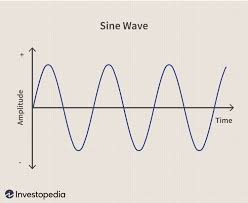
\includegraphics[width=\textwidth]{figures/sinwave.jpg}
		\caption{Sine Wave}
		\label{fig:1}
	\end{subfigure}
	\hspace{20mm}
	\begin{subfigure}[b]{0.4\textwidth}
		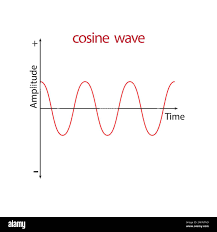
\includegraphics[width=\linewidth]{figures/cosinewave.png}
		\caption{Cosine Wave}
		\label{fig:2}
	\end{subfigure}
\caption{The Sine and Cosine waves}
\label{wave}
\end{figure}

Table can be drawn in \LaTeX using the following code.
\begin{table}[h!]
	\centering
	\caption{test table}
 \label{tab:testtable}
	\vspace*{5pt}
	\begin{tabular}{|c|c|c|}
		\hline
		Sl. No & Item 1 & Itm 2 \\ \hline
		1      & 37     & 45    \\ \hline
		2      & 42     & 23    \\ \hline
		3      & 47     & 1     \\ \hline
		4      & 52     & -21   \\ \hline
		5      & 57     & -43   \\ \hline
		6      & 62     & -65   \\ \hline
		7      & 67     & -87   \\ \hline
		8      & 72     & -109  \\ \hline
		9      & 77     & -131  \\ \hline
		10     & 82     & -153  \\ \hline
	\end{tabular}
\end{table}
Table referencing. Table \ref{tab:testtable} represents the testing values. 

%%********************Chapter 3**********
\chapter{\uppercase{Results and Discussion}}
Results here



%%********************Chapter 4**********
\chapter{\uppercase{Conclusion}}
Conclusion here



%*********************************Appendix*******************	


\appendix
\addtocontents{toc}{\string\let\string\chapappname\string\appendixname}
\titleformat{\chapter}[display]{\bfseries\filcenter}{\huge\appendixname{} \thechapter}{6ex}{\Huge\thispagestyle{empty}}

\fancyhead[L]{\slshape Appendix \thechapter} 
\fancyhead[R]{\nouppercase{ \slshape \footnotesize \leftmark}}

\chapter{ Sample Appendix 1}
Appendix A contents here

\chapter{Sample Appendix 2}
Appendix A contents here


%%********************References**********
%%****This template uses IEEE bibliography style
% The bib file references.bib can be found in the folder. Include the references in the bib file in BibTeX format. A quick video to generate the BibTeX file can be found at   % http://bit.ly/bibtex7
%
\bibliography{references}
\newpage


%************************List of Publications**********************

%If any publications pls add here
\listofpapers
\label{lop}
%\nobibliography{lop}
%\bibliographystyle{unsr}
\begin{enumerate}[{I. }]\bfseries
	\item \textbf{JOURNAL PUBLICATIONS} \\
	 	\begin{enumerate}[{1. }]\normalfont
		      \item author name (year)  
                      \newblock title  of paper
		           \newblock {\em name of journal}, volume,page number as pp., (year)
                      \newblock{doi}
            \end{enumerate}
% 	\item \textbf{REFEREED JOURNALS (Others)} \\
	\item \textbf{BOOK CHAPTER AND CONFERENCE} \\
            \begin{enumerate}[{1. }]\normalfont
                \item author names (year)  
                      \newblock title of paper
		           \newblock {\em conference/book name},publishers, page number, (year)
            \end{enumerate}
    \end{enumerate}            
\end{document}